\section{Anwendungsfälle}
\subsection{Sequenzdiagramm Simulator}

\begin{figure}[H]
\centering
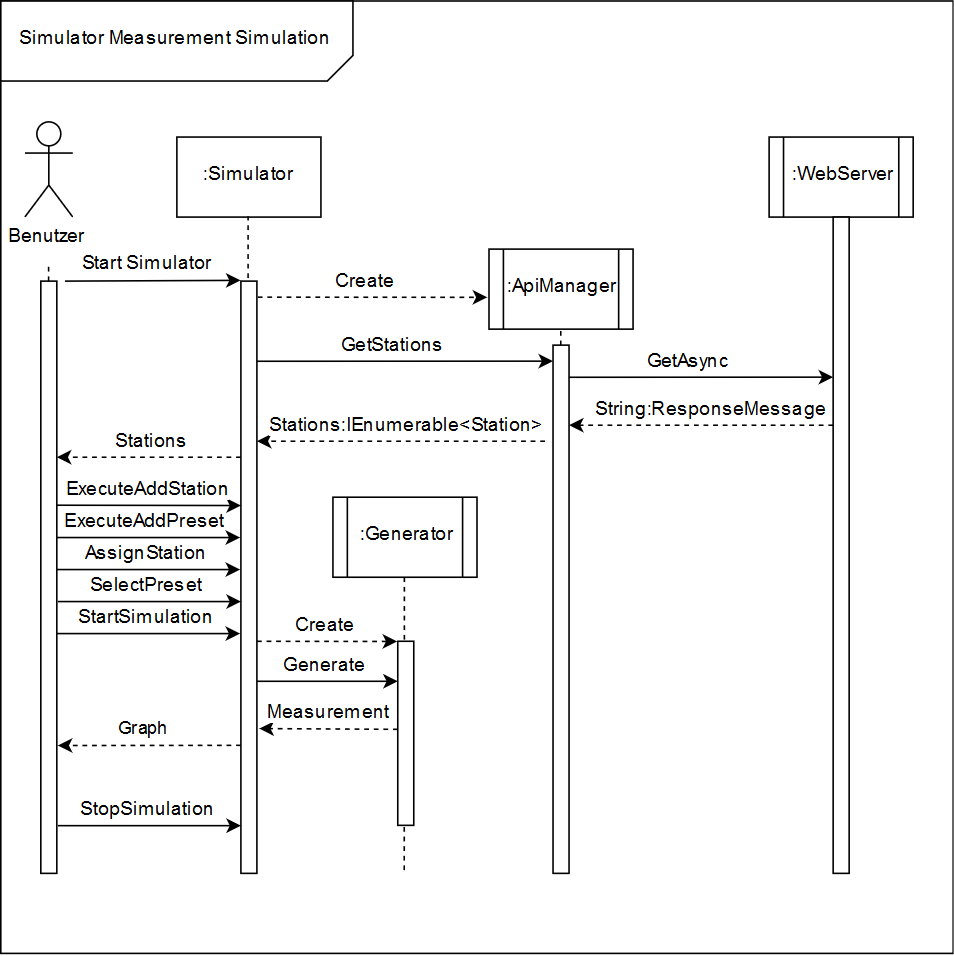
\includegraphics[scale=0.4]{pictures/sequence/Sequence_simulator_full.png}
\caption{Sequenz Diagramm Simulator}
\label{fig:Wetr.Simulator.Wpf-sequence}
\end{figure}
\raggedright

\subsubsection{Beschreibung}
Dem Anwender werden beim Start des Simulators alle verfügbaren Stationen angezeigt die zuvor mithilfe des \textit{ApiManager} geladen wurden. Der \textit{ApiManager} schickt einen request an den Webserver und liefert die Stationen an den Simulator zurück. Danach hat der Anwender die Möglichkeit diese Stationen für die Auswahl zu verwenden. Im nächsten Schritt kann der Anwender ein sogenanntes 'Preset' erstellen. Bei einem 'Preset' kann der Anwender festlegen welche Messwerte simuliert werden sollen und kann die Stationen die diese simulierten Messwerte erhalten bestimmen. Als letzten Schritt kann der Anwender die Simulation mit einem ausgewählten Preset starten oder stoppen. Der \textit{Generator} schickt dabei die generierten Daten mithilfe des \textit{ApiManager} Messwerte an den Webserver.


\newpage

\subsection{Sequenzdiagramm Cockpit}


\begin{figure}[H]
\centering
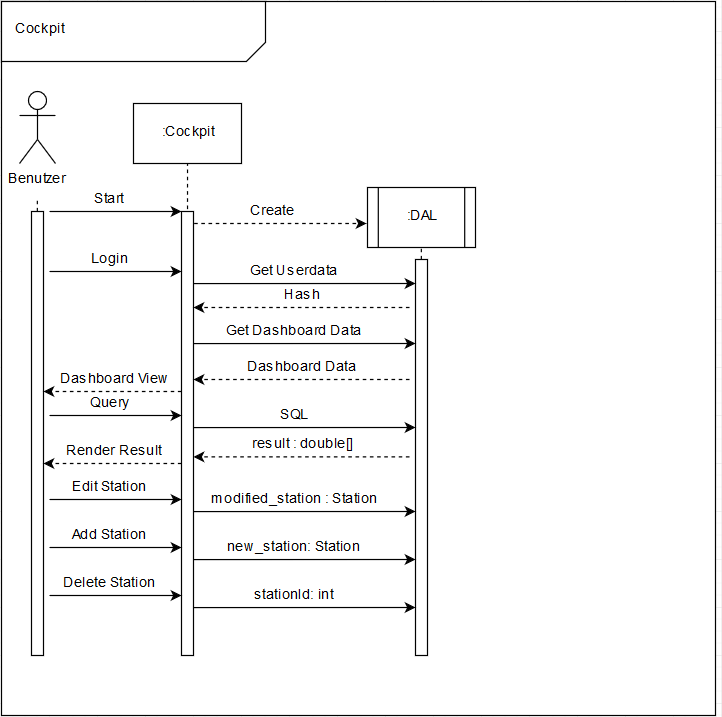
\includegraphics[scale=1.2]{pictures/sequence/Sequence_cockpit_full.png}
\caption{Sequenz Diagramm Cockpit}
\label{fig:Wetr.Cockpit.Wpf-sequence}
\end{figure}
\raggedright

\subsubsection{Beschreibung}

Beim Start des Cockpits muss sich der Benutzer zuerst mit den Benutzerdaten einloggen. Daraufhin frägt die Business Logic des Cockpits den Passworthash ab um ihn zu vergleichen. Bei erfolgreichem Einloggen werden diverse Daten abgefragt, wie z.B Anzahl der Stationen und Messdateb bzw. Wochenrückblick für Temperatur und Regenmenge. Diese Daten werden im Dashboard angezeigt. Wenn der Benutzer eine Messdatenabfrage tätigt, wird diese in einen SQL-String umgewandelt und im Data Access Layer ausgeführt. Das Ergebnis wird in einem Chart angezeigt. Beim Erstellen bzw. Löschen einer Station wird die neue/geänderte Station an den DAL geschickt und dort persistiert. Wenn eine Station gelöscht werden soll, reich es aus, die StationId zu schicken.